\chapter{\label{behaviour} Driving behaviour with optogenetics}

\minitoc

% Make sure you check the flow of this and that all the relevant information is included. I'm not 100 percent sure when writing that everything is there for a totally naive reader.

% The reference to the 1p figure panels are a little out of order too not sure I care

As detailed in the introduction, driving behaviour directly with experimentally controlled stimulation of neurons provides a unique window into neural computation, as recorded neurons by definition ignite the observed behaviour. Previously, this has been achieved in mice, by training animals, through operant conditioning, to learn the association between stimulation of neurons and reward \cite{huber_sparse_2008, houweling_behavioural_2008, histed_cortical_2014, dalgleish_how_2020, gill_precise_2020}. Two-photon holographic photostimulation is an ideal modality through which to drive neurons and ignite behaviour, as it allows for activation of a predefined number of neurons in a specific brain region which can be varied on a trial by trial basis. However, this major advantage of two-photon optogenetics is also a drawback with respect to driving behaviour, as the maximum number of neurons that can be activated simultaneously is on the order of 100. Hence, naive mice need first to be primed with more widespread activation to learn the task, before the number of cells is dialed down to the number attainable by two-photon activation. This has previously been achieved by training mice to respond to widefield "one-photon" optogenetics delivered by an LED \cite{dalgleish_how_2020, gill_precise_2020}.

Here, I developed a fully automated protocol for training mice to learn the association between photostimulation and reward, with mice reporting detection of the stimulus by licking a spout to receive a water droplet. Animals were trained initially through one-photon photostimulation with an LED. Mice learned to respond to activation of sequentially fewer neurons by reducing the LED power in a step-wise fashion when mice successfully learned to respond to a given power. Once mice had successfully learned the task at the lowest power level, in which only a few hundred neurons are likely activated \cite{huber_sparse_2008} they were transitioned to two-photon version of the task. Below is presented the structure of both versions of the task, as well as behavioural results. 

\section{One-photon photostimulation}

Mice expressing the opsin C1V1-Kv2.1, as well as the calcium indicator GCaMP6s, were trained on the one-photon version of the task (Figure \ref{fig:1-photon-behaviour}A), before being moved to the two-photon version. Although the two-photon stimulation light source is infrared and thus not detectable by the mouse retina, the 595 nm LED used in one-photon training is within the mammalian visual range \cite{peirson_light_2018}. Minimal light proofing was installed in behavioural training boxes; hence it is important to rule out that mice are detecting visual cues rather than photostimulation. The opsin C1V1-Kv2.1 is strongly activated by 595 nm LED stimulation \cite{yizhar_neocortical_2011, chettih_single-neuron_2019}, and we compared the behavioural performance of mice expressing this opsin in S1 to control mice which did not express an opsin activated by 595 nm light. Other than the virus injected, both opsin expressing and control mice were subjected to identical experimental conditions. 

A fully-automated training protocol was employed to maximise repeatability; this is detailed fully in materials and methods. Briefly, two trial types were delivered to the mice: go trials, in which LED stimulation was delivered, and catch trials in which no stimulation was delivered. 

The stages of the automated one-photon training protocol are shown in Figure \ref{fig:1-photon-behaviour}B. Naive mice initially learned to perform the task by pairing one-photon stimulation with reward regardless of the animal's response. This reward, delivered when the mouse did not make a behavioural response to the stimulation, is referred to as the auto-reward. As the reward was not delivered until the end of the response window, the trial outcome could still be scored according to Figure \ref{fig:1-photon-behaviour}E. Mice that scored 3 consecutive hits during the all trials auto-rewarded phase were transitioned to the active phase of the task in which the trial outcome was scored in the same way, but no auto-reward was delivered. Often however, particularly during the early stages of active training, mice began to fail to respond to stimulation. To refresh animals on the task, after 3 consecutive missed trials, an auto-reward was delivered on the subsequent go trial. We found a single auto-reward was enough to fully automate the training protocol and eliminate any manual intervention. 

The structure of a single trial is shown in Figure \ref{fig:1-photon-behaviour}C. To initiate a trial, mice had to withhold licking for a pseudorandomly sampled interval of 4-6 seconds. This eliminated repeated temporal structure from the task and reduced the chance of rewards by habitual licking. Trials were separated by a fixed 5 second inter-trial-interval. A 1 second response window was used to score the trial outcome. Licks during the response window were scored as hit and false positive for go and catch trials respectively, whereas withholding licking was scored as miss and correct rejection for go and catch trials respectively (Figure \ref{fig:1-photon-behaviour}E). 

 We began training by delivering high intensity LED stimulation (10 mW) and reduced the power as mice progressed through training (Figure \ref{fig:1-photon-behaviour}B,D). To automate power reductions, we used the d' metric \cite{brophy_alternatives_1986} to quantify behavioural performance (see materials and methods). This metric measures the animal's detection rate while controlling for baseline licking bias (the probability of responding in catch trials). We used a conservative threshold of d' > 2 which mice needed to exceed before they were transitioned to the next power level.
 
 We quantified the behavioural performance of opsin expressing mice and compared this to controls. First, we compared the number of trials required for mice to complete the first stage of training, recording three consecutive hit trials (Figure \ref{fig:1-photon-behaviour}F). On average, opsin expressing mice required fewer trials to reach this criterion (mean=247, std=223, N=14) compared to control mice (mean=365, std=83, N=4), however this difference was not significant (p=0.12 Mann-Whitney U test). Next, we compared the number of trials both cohorts took to complete the task (Figure \ref{fig:1-photon-behaviour}G,H), achieving d' > 2 on the lowest LED power level (0.1 mW). Opsin expressing mice required significantly fewer trials to reach this criterion (mean=667, std=206, N=14) compared to control mice (mean=1230, std=187, N=4) (p=0.005 Mann-Whitney U test). Finally, we compared the d' across all sessions recorded for both cohorts (Figure \ref{fig:1-photon-behaviour}I). Sessions recorded from opsin expressing mice had a significantly higher d' (mean=0.71, std=0.73, N=35) compared to control mice (mean=0.28, std=0.49, N=25) (p=0.006 Mann-Whitney U test).
 
\begin{figure}[h]
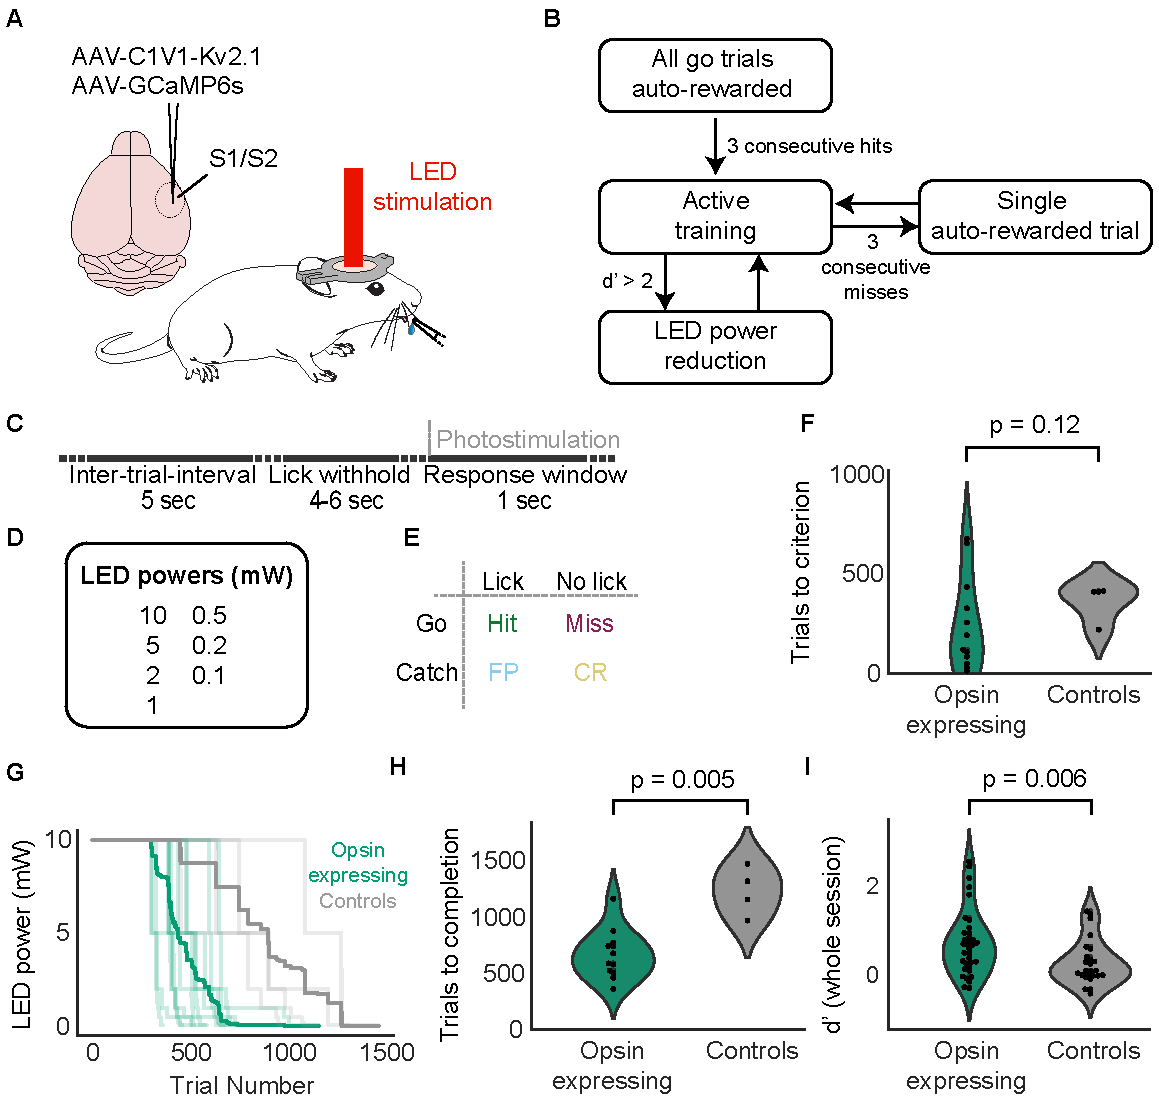
\includegraphics[scale=0.75]{figures/1-photon-behaviour.pdf}
\caption[\textbf{One-photon behavioural training.}]{
\textbf{One-photon behavioural training.}
\textbf{(A)} Schematic of the behavioural training setup. \textit{Left:} Viral injection performed in opsin expressing mice. \textit{Right:} Mice were headfixed and photostimulation was performed with an LED. A lick spout was placed within reach of the tongue, through which the animal reported perception of photostimulation by licking and received a water reward. \textbf{(B)} Steps in the fully automated training protocol. \textbf{(C)} Temporal structure of a single trial.  \textbf{(D)} LED powers used in the training. Mice started on 10 mW and were sequentially stepped down until they completed the task at 0.1 mW).  \textbf{(E)} Behavioral response matrix showing possible trial outcomes. \textbf{(F)} Number of trials required for mice to reach criterion (three consecutive hit trials) and complete the first stage of the task. Each point shows an individual mouse. \textbf{(G)} Ladder plot showing the LED power delivered to each mouse after a given number of trials. Thin transparent lines show individual mice and thick opaque lines show the average of the cohort. Mice were removed from the average calculation once they completed the task. Mice understood the task quicker if their ladder reached lower power levels after fewer trials. \textbf{(H)} Number of trials to complete the task for opsin expressing and control mice. Each point is an individual mouse. \textbf{(I)} d' across the whole session (for all power levels). Each point is an individual session.
} 
\label{fig:1-photon-behaviour}
\end{figure}

\section{Two-photon photostimulation}

Mice were headfixed and an objective lens was placed, immersed in water, over the cranial window. The same objective lens was used to deliver two-photon photostimulation and perform two-photon calcium imaging (Figure \ref{fig:2-photon-behaviour}A) (See \ref{res2}). The structure of the two-photon task is broadly the same as the one-photon (Figure 2\ref{fig:2-photon-behaviour}D,E). However, on go trials, we directly targeted photoresponsive S1 neurons with two photon photostimulation (see \ref{res2}). In addition, on catch trials, although we did not deliver photostimulating light to the brain, we moved all optical components to mimic the auditory component of go trials, meaning the animal could not perform the task from auditory queues alone. Mice were only auto-rewarded for a single trial if they recorded three consecutive miss trials. Photoresponsive S1 neurons were identified before the onset of behaviour, by photostimulating all opsin expressing neurons, in groups of 20, to find cells responsive to photostimulation.

Mice began on a version of the task with two trial types, where go and catch trials were initiated with equal probability. On all go trials, 150 S1 neurons were photostimulated (Figure \ref{fig:2-photon-behaviour}B). Once mice achieved a d' > 1.5 across the entire session, they were transferred to the main version of the task, which generated the data included in all further plots.

The main version of the task introduced a third trial type, not present for initial training. Between 5 and 50 photoresponsive S1 neurons were stimulated on this trial type (Figure \ref{fig:2-photon-behaviour}C) (see materials and methods). The behaviour of an animal on a single session is shown in Figure \ref{fig:2-photon-behaviour}F. The lick raster indicates more reliable licking behaviour and a greater propensity to score a hit trial, when a greater number of neurons were stimulated.

The number and identity of cells stimulated was varied randomly on a trial by trial basis (see materials and methods), generating a psychometric curve (Figure \ref{fig:2-photon-behaviour}G) which demonstrates that stimulating a greater number of neurons more robustly drove licking behaviour, and that the 50\% point of the psychometric curve fit across all sessions (N=10) is 23 neurons (95\% CI: 19 28), in accordance with previously published findings \cite{dalgleish_how_2020}. Therefore, by varying the identity and number of cells stimulated trial by trial, we delivered stimuli spanning the perceptual threshold of the animal, and ensured that the animal detects activity across the recorded population of S1 neurons rather than overtraining mice to report activity in a few specific neurons.

\begin{figure}[h]
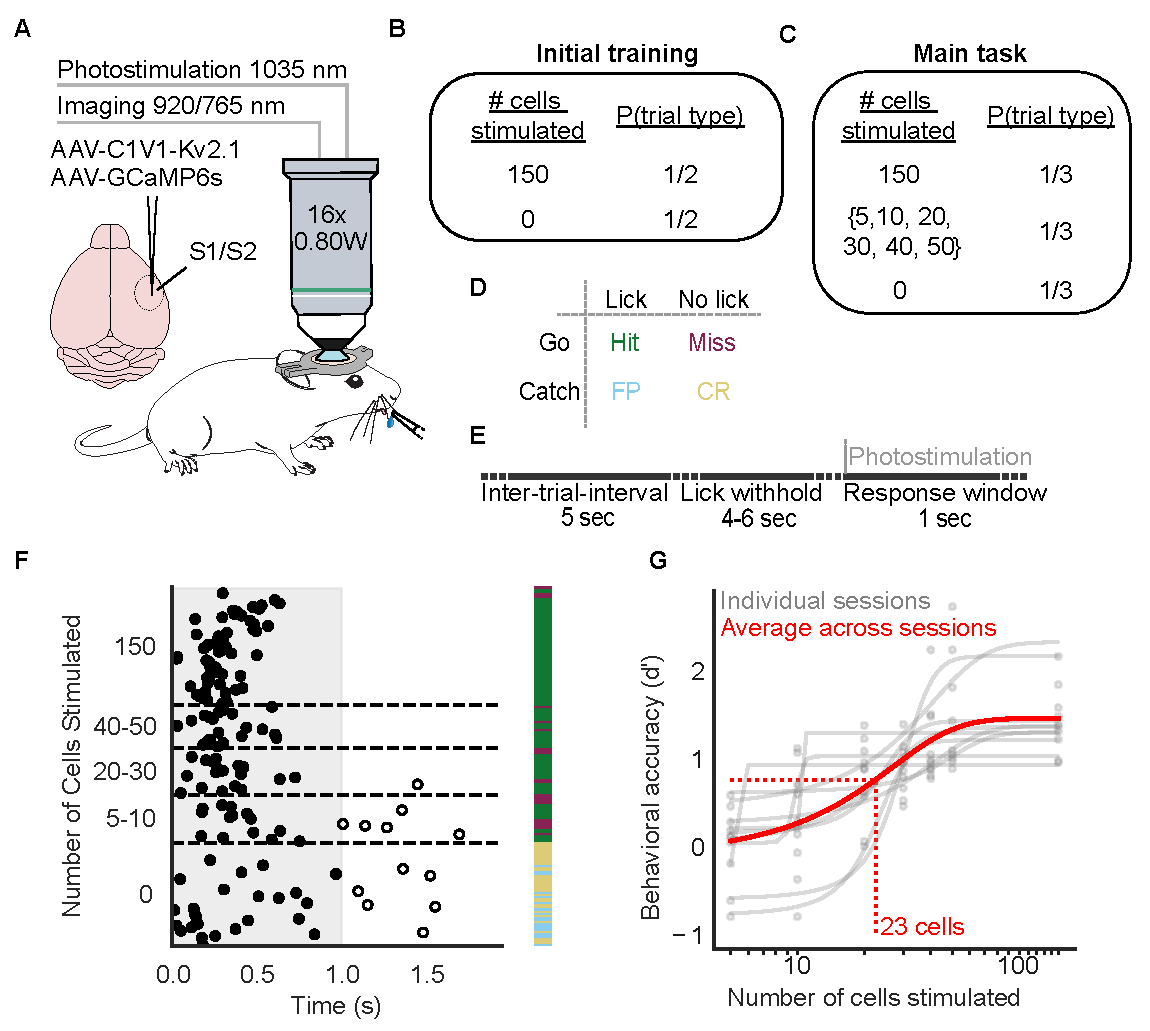
\includegraphics[scale=0.78]{figures/2-photon-behaviour.pdf}
\caption[\textbf{Two-photon behavioural training.}]{
\textbf{Two-photon behavioural training.}
\textbf{(A)} Schematic of experimental setup. \textit{Left}: viral strategy for expression of GCaMP6s and C1V1-KV2.1-mScarlet in S1 and S2.  \textit{Right}: mice with a cranial window installed over S1 and S2 were headfixed under a two-photon microscope. A lick spout was placed within reach of the tongue, through which the animal reported perception of photostimulation by licking and received a water reward. \textbf{(B)} Trial types for the initial stage of two-photon photostimulation training. \textbf{(C)} Trial types for the main task.  \textbf{(D)} Behavioral response matrix, colour code matches that in F. \textbf{(E)} Timing of a single behavioral trial. \textbf{(F)} Example lick raster from a single session sorted by number of cells stimulated and by time within each bin. Each row of the plot shows the first lick within an individual trial. Filled circles are licks occurring within the response window, open circles are licks occurring after the response window closes. The colourbar shows the outcome of the trial as defined in the behavioral response matrix. \textbf{(G)} Psychometric curves showing behavioral performance (d’) as a function of the number of cells photostimulated. Each grey point is the d’ computed for a given number of cells stimulated for an individual session and each grey line is a logistic function fit for an individual session. The red solid line shows the fit for all data points across all sessions (N=10 sessions; N = 5 mice). The red dashed line shows the 50\% point from the fit across all sessions. 
} 
\label{fig:2-photon-behaviour}
\end{figure}

In sum, this chapter demonstrates that I, alongside my colleagues, was able to develop a preparation in which experimentally controlled neural activity causally drove behaviour. Progression through the stages of training were automated, maximising repeatability and minimising human intervention. As explored in the next sections, this behavioural framework means that neural activity, causally underpinning behaviour, can be recorded, with single cell resolution, both locally and after propagation downstream.